% !TEX root=../main.tex
\section{Network Approach}
\label{sec:network}
The end goal of our project was to get the TurtleBot to follow a track purely using an image input to a neural network.
This section describes the architecture and training methods used to train a control network for the TurtleBot.

\subsection{Network architecture}
We experimented with multiple architectures, including a simple convolutional neural network (CNN), and a ResNet~\cite{ResNet}, but we eventually decided to use the DenseNet as our base architecture~\cite{DenseNet}.

\begin{figure}[hbt]
  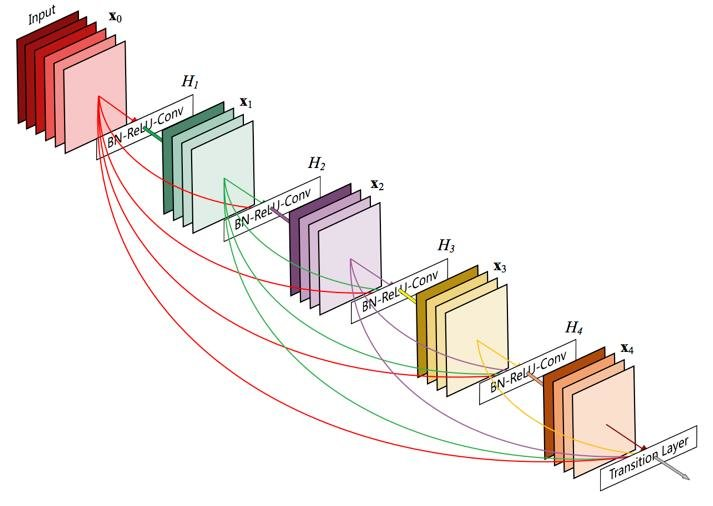
\includegraphics[width=\columnwidth]{figures/densenet}
  \caption{DenseNet architecture}
  \label{fig:densenet}
\end{figure}

The Densenet is a network architecture with densely connect convolutional
blocks, as seen in Figure~\ref{fig:densenet}. The DenseNet architecture is
unique because of the densely connected skip connections across multiple
convolutional blocks, which allows the architecture to re-use features
throughout the network. Accordingly, it has achieved better results than the
ResNet architecture on benchmarks such as ImageNet with a smaller memory footprint.

We used a pre-trained model for the DenseNet convolutional blocks, and added three linear layers with dropout to train the TurtleBot control using the DenseNet features.

\subsection{Network Training}
We used supervised, imitation learning to train the control network. We
collected data by driving the TurtleBot around multiple tracks on different
ground surfaces and matched RGB camera images to angular velocity command
outputs. We initially used the classical vision control method to gather data on
a single track, then diversified the data by manually driving the TurtleBot around other varied tracks and surfaces.

Using the image-command pairs, we trained the neural network to predict the
appropriate command for each input image. We trained the network on about 7
epochs of 15,000 image-command pairs.

\subsection{Continous Control}
Ideally, we would like the network to be able to predict a continous control
output given an input image. We allowed the network output to range from -1 to 1
radians per second. A simple way to limit the control effort was to use a
hyperbolic tangent function as the final activation on our linear layer output
layer.

After multiple attempts at training the network to predict a continouous output,
we were able to get some success, but the TurtleBot had a hard time making sharper turns and would often drive straight off the course instead of making the turns. In general, the control was underactuated.

\begin{figure}[hbt]
  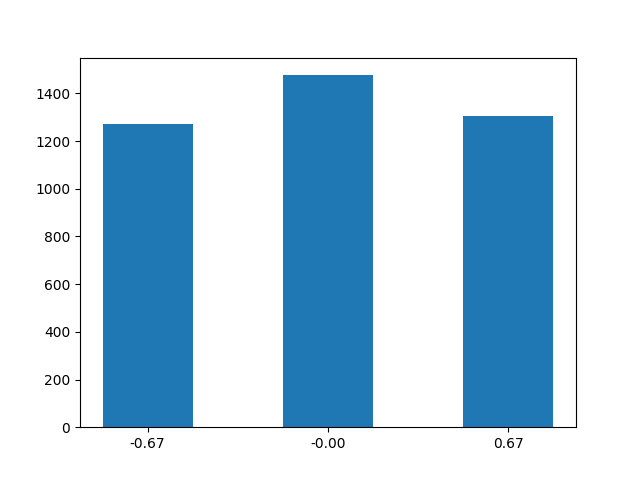
\includegraphics[width=\columnwidth]{figures/data_histogram}
  \caption{Histogram of the omega commands for the training data used.}
  \label{fig:data_hist}
\end{figure}

We assume that the issue was a data problem, so we plotted a rough distribution
of the data, as seen in Figure~\ref{fig:data_hist}. The data is centered about
zero and has a larger proportion of commands close to zero than it does further
away. It seems as though the network was able to quickly decrease the loss by
driving the control close to zero, causing the TurtleBot to default to slower
angular rates. The problem was then magnified because the TurtleBot would fail
to turn sharply, placing itself in a situation that it had not seen before and could not recover from.

To overcome this issue, we decided to try using an architecture with discrete
outputs and treat it as a classification problem. Some other potential solutions
to our problems could have included augmenting the data to include more
off-center scenarios or to gather data with more variety, including the corner
cases where the TurtleBot needs to recover from poor control or poor initial conditions.

\subsection{Discretized Control}
As a simple solution to the difficulties we faced when using continous control,
we decided to discretize the control by binning the allowable angular rate
values and using the midpoint of each bin as the representative angular rate
value for that bin. We used 5 bins to keep the classification problem simple,
but still have enough control authority to navigate sharper turns. With five
bins, the allowable control outputs were -0.8 (hard left), -0.4 (left), 0.0
(straight), 0.4 (right), and 0.8 (hard right) radians per second. Neural
networks are often better suited for classification problems and by using a cross-entropy loss function instead of the mean squared error loss, the network lost the incentive to center commands near zero, but instead was required to classify each image in the correct command bin.

This approach proved to be much more successful and we were able to replicate and eventually surpass the performance of the classical method.
